% Dokumentklassen sættes til memoir.
% Manual: http://ctan.org/tex-archive/macros/latex/contrib/memoir/memman.pdf
\documentclass[a4paper,10pt]{article}
\usepackage{pdfpages}
\usepackage[a4paper]{geometry}
% Danske udtryk (fx figur og tabel) samt dansk orddeling og fonte med

% danske tegn. Hvis LaTeX brokker sig over æ, ø og å skal du udskifte
% "utf8" med "latin1" eller "applemac". 
\usepackage[utf8]{inputenc}
\usepackage[english]{babel}
\usepackage[T1]{fontenc}
% \usepackage{setspace}
%\doublespacing
% Matematisk udtryk, fedes fymboler, theoremer og fancy ting (fx kædebrøker)
\usepackage{amsmath,amssymb}
\usepackage{bm}
\usepackage{amsthm}
\usepackage{tikz}
%\usepackage{mathtools}
% Kodelisting. Husk at læse manualen hvis du vil lave fancy ting.
% Manual: http://mirror.ctan.org/macros/latex/contrib/listings/listings.pdf
\usepackage{listings}
\usepackage{verbatim}
\usepackage{hyperref}

\usepackage[section]{placeins}

% Fancy ting med enheder og datatabeller. Læs manualen til pakken
% Manual: http://www.ctan.org/tex-archive/macros/latex/contrib/siunitx/siunitx.pdf
%\usepackage{siunitx}
% Indsættelse af grafik.
\usepackage{graphicx}
%\usepackage{bussproofs}
\usepackage{natbib}

\usepackage[font=small,labelfont=bf,labelsep=space]{caption}
\usepackage{siunitx}
\sisetup{output-exponent-marker=\ensuremath{\mathrm{E}}}
%Install abstract package and and \usepackage{abstract}
\renewcommand{\abstractname}{Abstract}    

% Reaktionsskemaer. Læs manualen for at se eksempler.
% Manual: http://www.ctan.org/tex-archive/macros/latex/contrib/mhchem/mhchem.pdf
%\usepackage[version=3]{mhchem}
\author{Christian Budde Christensen, 20103616\\Nicklas Pingel, 20102222\\Lukas Walther, 20107539}
\title{Advanced Data Structures}
\date{\today}
\begin{document}
\maketitle
\tableofcontents 
\clearpage

\section{Introduction}
In this report, we will experiment with and analyze the running times of our implementations of \texttt{FIBONACCI-HEAP} and \texttt{BINARY-HEAP}. We also argue about the worst-case behaviour of the implemented methods. The two different implementations of a priority-queue are then used in Dijkstra's algorithm, computing single-source shortest paths on different types of graphs. The objective of these experiments is to analyze, wether or not the amortized running time of $O(1)$ of \texttt{FIBONACCI-HEAP}'s decrease-key operation leads to a decrease in running time, when used by Dijkstra's algorithm.

\section{Implementation}
Both Heaps are implemented in \texttt{C++} with an Object Oriented approach. The heaps inherit a \texttt{Heap} interface and the nodes a \texttt{Node} interface. This style enables us to create generic tests and easily provide our Dijkstra algorithm with different heap implementations. Furthermore, impementing our heaps in this OO manner provides a nice level of code tranparency and less redundant code.% without loss of speed or corruption of runtime, as it might be the case had we decided to implement the heaps in \texttt{Java}.%%% det her har ikke noget at gøre med java.

Fibonacci heaps are implemented very much like in Introduction to Algorithms \cite[Chapter 19]{clrs}. Fibonacci Heap's nodes are arranged in doubly linked circular lists, where each node has a pointer to its parent, one child, and the nodes left and right to it. We keep a pointer to the \texttt{minRoot} node, which together with its siblings make up the forest. There are no relevant differences in our implementation, compared to Fredman and Tarjans \cite{fredman} or CLRS \cite{clrs} version, other than that we use the more object-orientated style of programming.

Binary heaps are implemented with a pointer-based datastructure, instead of organizing the nodes implicitly within an array. This means, to find the last node correctly, or find out where to insert a new node, without using $O(n)$ time, we use decimal to binary conversion to compute a path trough the heap to the position that is needed. This can be achieved in $O(\log(n))$ time, without changing the established asymptotic running time. We chose to use a pointer-based structure, to make the heaps more comparable to each other.
The implemented methods are \texttt{MakeHeap}, which is just the constructor of an object, \texttt{Insert}, \texttt{DeleteMin}, \texttt{DecreaseKey}, \texttt{FindMin} and \texttt{Remove}. The \texttt{Meld} method is only partially implemented, and is not considered or used in this report.%% As we will show later, when the different heap's methods have the same asymptotic behaviour, they also achieve the same measured running time %%

\section{Worst Case Analysis}
The following is a worst case analysis of each function in the implementations of Fibonacci Heap and Binary Heap.
The heap property refers to the invariant, that no child node can have a strictly smaller key than its parent.
%Following is worst case analazys of each function in our impoementations of the Fibonacci Heap and the Binary Heap. The heap property refers to the invariant that no child node must have a smaller key than its parent.
\subsection{Fibonacci Heap}
This heap has been implemented as a \texttt{C++} class with the functions analyzed below. Let $n$ denote the number of elements in the heap and \texttt{minRoot} the pointer to the node containing the smallest key in the heap. %Let $H$ denote the current heap, $t(H)$ the number of trees in $H$, $m(H)$ the number of marked nodes, \texttt{minRoot} the pointer to node containing the smallest key in the heap and $n$ the number of nodes in the heap. 
\subsubsection*{MakeHeap}
The \texttt{MakeHeap} function, taking no arguments, creates an empty heap, and is implemented as the class constructor. Because no trees or nodes are created, this operation takes $O(1)$ running time.
\subsubsection*{FindMin}
The \texttt{FindMin} function returns \texttt{minRoot}, kept in the heap. The pointer can be updated by \texttt{Insert}, \texttt{DeleteMin} or \texttt{DecreaseKey} when appropiate. Returning the pointer takes constant time ($O(1)$). The structure of the heap isn't changed in any way.
\subsubsection*{Insert}
The \texttt{Insert} function takes two arguments, a key and a payload. The heap then constructs an instance of \texttt{Node} with the given properties, and inserts it as a tree with a single node. If the newly inserted node, \texttt{n}, has a smaller key than \texttt{minRoot}, \texttt{n} becomes the new \texttt{minRoot}.
Inserting the new tree takes constant time. The trees are being kept in a doubly linked list, and inserting an element into such a list is achieved with a constant amount of pointer operations. Updating \texttt{minRoot} also takes constant time, because we only have to compare two values and update a pointer. Therefore the worst case running time must be $O(1)$.
\subsubsection*{DeleteMin}
When deleting \texttt{minRoot}, we have to insert all \texttt{minRoot}'s children into the forest of trees. This is done in constant time with pointer arithmatic on the doubly linked lists containing the children and the forest.

The we iterate through all trees in the forest, and store them in an array according to their rank. When two trees having the same rank are found, we meld the two trees together, keeping the one with the lowest key on top, and inserting the other on as a child. This has to be done iteratively, as we now have a node with a bigger rank, and we could have another node of the same rank. There can be up to $\log n$ iterations of melding trees together, as the maximum rank is bounded by $\log n$.

For iterating through all the trees, we can use op to $n$ iterations, as all elements could be trees of size one, thus being siblings in the forest. In this case though, the amount of recursions is limited. We can only have $\frac{1}{2} n$ recursions of depth equal or bigger to 1, because only every second node we traverse can possible give rise to recursion. Likewise, only every fourth node can give rise to recursion of depth 2 and only every eight node can give rise to recursion of depth 3. We can express this as $n + \frac{1}{2}n + \frac{1}{4}n + \frac{1}{8}n + ...$, which in turn sums up to $2n$, which is $O(n)$.

In the next loop, we search for the new \texttt{minRoot}, which can at most take $O(\log n)$ time, because there is only one tree of every rank left.

Therefore the worst case running time for \texttt{DeleteMin} is $O(n)$.

%* Deletes min root and adds children as new roots
%* Iterate throug all roots and meld them if they have same rank
%* Worst case runtime is O(n) following all t(H) could be n

%* Amortized: Delete adds max O(log(n)) new trees (following a node can have rank max log(n))
%* ... 
%* Profit 

%When this function is called, an array of pointers is created. The array is of size $O(\log(n))$. Then This has a cost less or equal max degree of any node in our Fibonacci heap($d_n$) + 1. Lets suppose we start with $k$ trees in our doubly linked list of roots, and perform $l$ link operations we then perform $k+l$ work, and end up with $k-l$ trees. The worst case for linking the heap would be $n$ elements in our doubly-linked list of roots, with none of these combined in a tree. $t(H)$ will be reduced by $k/2$, and we do not mark any nodes. The worst case is then $O(n)$. 

%For the amortized case we look at the potential change, given as $\Delta_i \geq -2l$. The amortized cost, of the $i$-th operation with respect to the potential function is $\hat{c_i} = c_i + \Delta_i \leq 2(k - l) + d_n + 1$. But will be $k - l\leq d_n + 1$ because we can have at most one tree of each rank so, $\hat{c_i}\leq 3d_n + 3 = O(\log n)$.

\subsubsection*{DecreaseKey}
Given a node $x$ and a key $k_x$, we set $x$'s key to be be $k_x$, only if $k_x$ is smaller than the key $x$ currently has.

If $x$ has a parent, $p_x$, we test, if the heap property is violated. If $x$'s key is now smaller than $p_x$'s key, we cut the connection between those two, and insert $x$ as a tree at the \texttt{minRoot} and unmark $x$.
Then we test if $p_x$ is marked. If $p_x$ is not marked, we mark it. Otherwise, we also cut $p_x$ from its parent and insert it at the \texttt{minRoot}, thus unmarking it. This is done with each parent we visit, until there is no parent left, or we reach an unmarked node.

The operation of cutting a node from its parent takes constant time. Inserting a tree in the doubly linked list also takes constant time. Therefore each iteration takes constant time. The height of the tree $x$ is a part of can at most be $\log n$. This means that we can visit at most $\log n$ parents in the worst case. This gives us a worst case behaviour of $O(\log n)$

%%We decrease the key of the node $x$ to the new key $k_x$, and if the heap property becomes violated, the node is cut from its parent. We also mark up the tree untill we hit a node or an unmarked node. For each cut we unmark a node when making the node a root.
%%
%%We increase $t(H)$ by $k$, the number of cuts and in the end mark at most 1, so $m(H)$ increase at most 1. The overall cost is computed as $c_i=1+k=O(k)$ where each cut operation takes $O(1)$. This will in the worst case, where we have $\log n$ number of nodes we need to cut yield a worst case running time of $O(\log n)$.

%%When we look at the amortized running time, we first look at the potential drop
%%\begin{align*}
%%t(D_i)-t(D_{i-1}) &= 1 + k, m(D_i)-m(D_{i-1})\leq -k+1\\
%%\text{potential drop, } \Delta_i &= 2(t(D_i)-t(D_{i-1}))+3(m(D_i)-m(D_{i-1}))\\
%%&\leq 2(1+k)+3(-k+1)\\
%%&= -k+5
%%\end{align*}
%%Thus we can see that the amortized cost, $\hat{c_i}$, of \texttt{DECREASE-KEY} is
%%\begin{align*}
 %% \hat{c_i} &= c_i + \Delta_i\\
  %%&\leq (1+k)+(-k+5)\\
  %%&= 6 = O(1)
%%\end{align*}
\subsection*{Delete}
Given a node $x$ we want to remove from the heap, we use \texttt{DecreaseKey} to set its key to be the lowest key of the heap, which ensures that \texttt{minRoot} points to $x$. We then call \texttt{DeleteMin}, which removes $x$ from the heap.
In the worst case, \texttt{DecreaseKey} takes $O(\log n)$ time and \texttt{DeleteMin} takes $O(n)$ times.  $O(\log n) + O(n) = O(n)$, therefore \texttt{takes} linear time in the worst case.

%%The worst case is bounded by the worst case of \texttt{DECREASE-KEY} plus the worst case of \texttt{DeleteMin}. By combining these we get $O(\log n) + O(n) = O(n)$ in the worst case. \texttt{DELETE} is also bound by the method's amortized time, $\hat{c_i}$

%%\begin{align*}
%%\hat{c_i} =& \text{ amortized cost of Decrease-Key}\\
%%&+\text{amortized cost of DeleteMin}\\
%%=& O(1) + O(\log n)\\
%%=& O(\log n)
%%\end{align*}


\subsection{Binary Heap}
The Binary-Heap implementation holds a pointer to the root of the heap and a pointer to the last element in the heap.
\subsubsection*{Make-heap}
As with Fibonacci Heap, we only construct the heap, but we do not construct any nodes. Because of this we have $O(1)$ running time.

\subsubsection*{FindMin}
Because of the heap property, the minimum element will always be present at the root of the heap. By keeping a pointer to the root, we can return this element in constant time. The worst case running time is therefore $O(1)$.

\subsubsection*{Insert}
Inserting an element into the heap is done by placing it as a new leaf of the heap, and bubbling up as long as the parent of the node has a bigger key. In the worst case, the node has to be placed at the root of the heap, thus making $\log n$ comparisons and exchanges to reach the top.
Placing the new node at at the bottom of the heap takes $\log n$ time, as we have to compute the path through the heap using decimal to binary conversion and then following the path from the root node. This takes $2\log n$ time. Thus the worst case running time for insertions is $O(\log n)$.

\subsubsection*{DeleteMin}
To delete the heaps top node, we replace it with the heaps last node. This step is done in constant time. Then we test wether the current top node has a bigger key than one of its children, if so, we exchange it with the child having the smallest key. This is repeated until the heap property is restored. We can bubble down at most $\log n$ times, at which point the node will not have any children left.
Therefore, \texttt{DeleteMin} has a worst case running time of $O(\log n)$.

\subsubsection*{DecreaseKey}
Given a node and a new key, we set the nodes key to be the new key, only if the new key is smaller than the current key. We then procede with testing wether or not the node has a smaller key than its parent, in wich case we let it bubble up, until the heap property is restored. This can at most be $\log n$ comparisons and exchanges, therefore \texttt{DecreaseKey} has a worst case running time of $O(\log n)$.
\subsubsection*{Delete}
Upon deletion of a given node, $x$, we first use \texttt{DecreaseKey} to set the key of $x$ to the lowest value in the heap (smaller than the root). We then use \texttt{DeleteMin} to remove the top node, which now is $x$.

The worst case for \texttt{Delete} is bounded by the worst case for \texttt{DecreaseKey} plus the worst case for \texttt{DeleteMin}. This gives us a $O(\log n) + O(\log n) = O(\log n)$ worst case running time.

\begin{table}
  \begin{center}
    \begin{tabular}{l|c|c}
      & Fibonacci Heap & Binary Heap \\
      \hline
      Make-Heap    & $O(1)$             & $O(1)$\\
      Find-Min     & $O(1)$             & $O(1)$\\
      Insert       & $O(1)$             & $O(\log n)$\\
      DeleteMin   & $O(n)$             & $O(\log n)$\\
      Decrease-Key & $O(\log n)$        & $O(\log n)$\\
      Delete       & $O(n)$             & $O(\log n)$
    \end{tabular}
    \caption{Worst case execution time for Fibonacci and Binary Heap}
    \label{worst-case-analysis}
  \end{center}
\end{table}


\section{Heap Experiments}
All experiments were run on a linux machine, using an x86\_64 Intel Xeon W3520 running at 2.67GHz. The computer is equipped with 24 GB of RAM of type DDR3. Experiments did not require more than 10 gigabyte of memory, so it is safe to assume that the swap would not be used by our programs. The processor has four physical cores, one of which was dedicated to running our experiments, so influence of other programs should be very small.

All programs were run using Linux Mint version 15. The \texttt{C++} program was compiled using \texttt{g++} version 4.7.3 with \texttt{-fexpensive-optimizations}, \texttt{-O3} and \texttt{-std=c++11} flags.

The program is compiled via a makefile and can be run with by calling \texttt{\.\/fibheap}. All measurements will be written to .csv files that can be opened with a texteditor or a spreadsheet program like Microsoft Excel or LibreOffice. We included our source-code and our results with this hand-in. The \texttt{.ods} files contain additional calculations like averaging and divison of running times and can be opened with OpenOffice or LibreOffice.

All experiments were timed with the \texttt{clock\_gettime} method from the \texttt{C++} standard library, which offers resolutions close to a few nanoseconds. The \texttt{CLOCK\_PROCESS\_CPUTIME\_ID} flag is used, which measures the CPU-time spent on running the program, instead of using real-world time, which could potentially be inflated by background processes.
All experiments write their results to different files. Care is taken to only measure the time spent computing the methods under observation, not the writing to files or generation of input or graphs.

\subsection{Fibonacci Heap}
\subsubsection{Insert}
{\bf Hypothesis}\\
We have that \texttt{FIBONACCI-HEAP-INSERT} inserts an element in $O(1)$ time. This means that when we perform $N$ insertions into a fibonacci heap we expect to measure a running time that increases linearly with the number of insertions.\\
This experiment consists of inserting $N$ elements into the heap. The element's keys range from $N$ to $2N$, which has no effect on the execution time of \texttt{FIBONACCI\--HEAP\--INSERT}, but is usefull for later experimentation with \texttt{FIBONACCI\--HEAP\--DECREASE\--KEY}.\\
In table \ref{fibonacci-insert-table}, we present the measured running times for \texttt{FIBONACCI\--HEAP\--INSERT} for $N$ elements.
\begin{table}
  \begin{center}
    \begin{tabular}{l|r|r}
      $N$ & measured insert time(s) & measured insert/N time(s)\\
      \hline
      10       & \num{5.971E-7}     & \num{5.971E-8}\\
      100      & \num{3.424E-6}     & \num{3.424E-8}\\
      1000     & \num{4.215E-5}     & \num{4.215E-8}\\
      10000    & \num{5.587E-4}     & \num{5.588E-8}\\
      100000   & \num{0.0056}       & \num{5.668E-8}\\
      1000000  & \num{0.0610}       & \num{6.100E-8}\\
      10000000 & \num{0.6070}       & \num{6.070E-8}
    \end{tabular}
    \caption{Bounds and measured running time}
    \label{fibonacci-insert-table}
  \end{center}
\end{table}\\
{\bf Conclusion}\\
The time spent per single insert operation varies around a constant factor. Even though the numbers do not form a horizontal line on the graph, they are in the same order of magnitude, excluding the possibility of an exponential growth. Graph \ref{fibonacci-insert-graph} gives a good impression of \texttt{FIBONACCI-HEAP-INSERT} running in constant time for a single element, as the number of elements to be inserted tenfold, the running time also tenfolds. Thus we can safely assume that the \texttt{FIBONACCI-HEAP-INSERT} method actually runs in constant time.

\subsubsection{DecreaseKey}
{\bf Hypothesis}\\
The amortized running time for \texttt{FIBONACCI-HEAP-DECREASE-KEY} is $O(1)$ and the worst case running time is $O(\log n)$. The experiment consists of a heap with $N$ elements with increasing keys from $N$ to $2N$, where \texttt{FIBONACCI-HEAP-DECREASE-KEY} is called with elements in decreasing order of their key, reducing their key by $N$, which means that the heap updates it's minimum element with each call. The expectation is, that after some calls to \texttt{FIBONACCI-HEAP-DECREASE-KEY}, the cost of calling \texttt{FIBONACCI-HEAP-DECREASE-KEY} will approach a constant, which implies that $N$ calls to \texttt{FIBONACCI-HEAP-DECREASE-KEY} will have an amortited running time of $O(N)$. In table \ref{fibonacci-decrease-key-table} we present the measured running times for \texttt{DecreaseKey} and the values divided by the size of the heap. These values are plotted in graph \ref{fibonacci-decrease-key-per-element}.
\begin{table}
  \begin{center}
    \begin{tabular}{l|r|r}
      $N$ & measured decrease time(s) & measured decrease time(s) /N \\
      \hline
      10       & \num{5.492E-7}     & \num{5.492E-8}\\
      100      & \num{3.590E-6}     & \num{3.589E-8}\\
      1000     & \num{3.244E-5}     & \num{3.245E-8}\\
      10000    & \num{3.195E-4}     & \num{3.200E-8}\\
      100000   & \num{0.0034}       & \num{3.434E-8}\\
      1000000  & \num{0.0372}       & \num{3.718E-8}\\
      10000000 & \num{0.3847}       & \num{3.847E-8}
    \end{tabular}
    \caption{Bounds and measured running time}
    \label{fibonacci-decrease-key-table}
  \end{center}
\end{table}\\\\
{\bf Conclusion}\\
The measurement divided by the number of \texttt{FIBONACCI-HEAP-DECREASE-KEY} calls approach a factor of \num{3.786E-8}, within a small margin of error, when we ignore the first measurement of size 10, as this is easily inflated due to its very short running time. We can safely conclude that the cost of each \texttt{FIBONACCI-HEAP-DECREASE-KEY} call is close to a constant factor, after many calls to the method, though one could still take measurements to find after how many calls in succession \texttt{FIBONACCI-HEAP-DECREASE-KEY} comes close to constant running time.

\subsubsection{DeleteMin}
{\bf Hypothesis}\\
The worst case running time for \texttt{FIBONACCI-HEAP-DELETE-MIN} is $O(n)$ and the amortized running time is $O(\log n)$. In this experiment, we start out with a heap of size $N$ and call \texttt{FIBONACCI-HEAP-DELETE-MIN} until the heap is empty. For this amount of delete-min operations, the total running time is expected to be $O(\log(N!))$. Due to the amortized running time, we expect $N$ \texttt{FIBONACCI-HEAP-DELETE-MIN} operations to perform much better than \[G(N) = \sum^N_{n=1} n = \frac{N(N-1)}{2}.\] The measured running times and theoretic values for $O(\log n)$ and $G(N)$ can be found in table \ref{fibonacci-delete-min}. These datapoints are visualized in graph \ref{fibonacci-delete-min-graph}\\\\
\begin{table}
  \begin{center}
    \begin{tabular}{l|r|r|r}
      $N$ & expected running time(s) & measured running time(s) & $G(N)$\\
      \hline
      10       & \num{20}           & \num{1.981E-6} & \num{45}\\ 
      100      & \num{522}          & \num{2.523E-5} & \num{4950}\\
      1000     & \num{8504}         & \num{0.000254} & \num{499500}\\
      10000    & \num{118261}       & \num{0.00383}  & \num{49995000}\\
      100000   & \num{1516460}      & \num{0.04043}  & \num{5E+9}\\
      1000000  & \num{18488855}     & \num{0.43195}  & \num{5E+11}\\
      10000000 & \num{218107833}    & \num{3.71978}  & \num{5E+13}
    \end{tabular}
    \caption{Bounds and measured running time}
    \label{fibonacci-delete-min}
  \end{center}
\end{table}\\\\
{\bf Conclusion}\\
The measured running times show that the running time increases at most at the same rate as the theoretical bound we expected and increases not at all like the worst-case bound for $N$ insertions. We can conclude that this implementation of \texttt{FIBONACCI-HEAP-DELETE-MIN} operates in the expected amortized bound of $O(\log n)$.

\subsection{Binary Heap}
\subsubsection{Insert}
In this section will we explore the running time of Binary-Heaps insert method. The running time is analyzed in two different ways. At first, we run a number of inserts accumulative and observe the total running time of $N$ \texttt{BINARY-HEAP-INSERT} operations. Then we analyze \texttt{BINARY-HEAP-INSERT} operations relative to the height of the heap and thereby to the number of iterations in the worst case.\\\\
{\bf Hypothesis}\\
To measure the running time, $N=10^k$ elements with decreasing key are inserted into the heap in succession to achieve worst-case behaviour. This is done 50 times to compute an average. Because the \texttt{BINARY-HEAP-INSERT} operation is done $N$ times in succession, we expect the running time to be the sum over the individual insert operation at any given size of the heap, which is called $n$.
Thus, we expect to measure a running time of the form: \[\sum^N_{n=1}\log n.\]
We have $\log(a)+\log(b)=\log(a\cdot b)$ so 
\begin{align*}
  f(N)=\sum^N_{n=1}\log(n)&=\log(1)+\log(2)+\cdots+\log(N)\\
  &=\log(1\cdot2\cdot3\cdots N)\\
  &=\log(N!)
\end{align*}

The numbers for $f(N)$ in table \ref{binary-insert-accumulative} are only approximate, as computing the faculty of numbers bigger than 100 is troublesome. The data measured this way can be found in table \ref{binary-insert-accumulative}.

In the second experiment, an emtpy heap is used, and elements are inserted layer by layer. To increase the height of the heap by one every time, we insert $2^k$ elements, where k is the height of the heap. Each element is inserted with a key that is smaller than the smallest key currently in the heap, which means that the element has to travel through the $k$ layers in the heap to reach the top. This is the worst case scenario for \texttt{BINARY-HEAP-INSERT}.

For each layer, we measure the time for running \texttt{BINARY-HEAP-INSERT} $2^k$ times and divide the running time by the numbers of elements inserted, which yields an average running time for the current height of the heap. This value is then divided by the current height of the heap, which results in the time spent per iteration. This time should come close to some constant, if insertion runs in $O(\log n)$ time.
The data for this experiment is shown in table \ref{binary-insert-layer}.
\begin{table}
  \begin{center}
    \begin{tabular}{l|r|r}
      $N$ & $f(N)$ & measured running time(s) \\
      \hline
      10       & 20         & \num{1.6487E-6}\\
      100      & 522        & \num{2.3691E-5}\\
      1000     & 8504       & \num{2.6033E-4}\\
      10000    & 118261     & \num{3.4728E-3}\\
      100000   & 1516460    & \num{4.1341E-2}\\
      1000000  & 18488855   & \num{0.4934}\\
      10000000 & 218107833  & \num{5.5171}
    \end{tabular}
    \caption{Bounds and measured running time}
    \label{binary-insert-accumulative}
  \end{center}
\end{table}
\begin{table}
  \begin{center}
    \begin{tabular}{l|r}
      Height of the heap & $\frac{\text{average running time (s)}}{\text{height}}$  \\ %:)
      \hline
     1 & 4.02436E-006   \\
     2 & 0.000000695    \\
     3 & 1.98740E-007   \\
     4 & 1.20565E-007   \\
     5 & 7.92507E-008   \\
     6 & 5.57850E-008   \\
     7 & 4.74929E-008   \\
     8 & 0.000000043    \\
     9 & 3.99142E-008   \\
     10 & 3.560906E-008 \\
     11 & 3.765503E-008 \\
     12 & 3.536233E-008 \\
     13 & 0.000000036   \\
     14 & 3.825133E-008 \\
     15 & 4.064006E-008 \\
     16 & 3.991053E-008 \\
     17 & 3.885869E-008 \\
     18 & 3.783860E-008 \\
     19 & 3.722322E-008 \\
     20 & 3.660788E-008 \\
     21 & 3.605462E-008 \\
     22 & 3.558514E-008 \\
     23 & 3.519494E-008 \\
     24 & 3.485190E-008 \\
     25 & 3.453128E-008  
    \end{tabular}
    \caption{Running time for insertions divided by the height of the heap. }
    \label{binary-insert-layer}
  \end{center}
\end{table}\\\\
{\bf Conclusion}\\
In graph \ref{binary-insert-accumulative-graph}, we plot the data for the proposed function and the measured running time on a doubly logarithmic graph, and we see, that they have the same tendency. We can safely discard the measured running times for 10 elements, as running times this close to single microseconds may easiliy be dominated by the constant factors. We observe that the running time increase at most at the same rate as the theoretical bound, this means that our measured running time conforms to the expected running time $O(\log N!)$. Hereby the running time of binary heap's insert conforms to the expected asymptotic running time $O(\log n)$.

The data for the second experiment is plotted in graph \ref{binary-insert-layer-graph}. Observe that after a height of 15, the running time divided by the number of layers in the heap gets close to a constant of about 3.4E-8. Therefore the total running time increases linearly with the number of layers in the heap. This confirms our hypothesis, that \texttt{BINARY\--HEAP\--INSERT} runs in $O(\log n)$ time.

%As expected, the number of comparisons for an insert operation is logarithmic in the size of the heap in the worst case. Comparing the running times for insertion divided by the number of comparisons in table \ref{binary-insert-single} shows some irregularities. At heap size of 10, 100, 10.000, 100.000 and 10.000.000 are close to the same constant, the values for heap sizes of 1.000 and 1.000.000 vary wildly. This can possibly be explained by the elements being compared sometimes being on few pages of memory, whilst other times being spread amongst multiple pages of memory, though we have no further data to back up this claim. %% DET HER ER RIMELIG USELESS NU.
\subsubsection{DecreaseKey}
{\bf Hypothesis}\\
The \texttt{BINARY\--HEAP\--DECREASE\--KEY} method has a worst case running time of $O(\log n)$ where $n$ is the current size of the heap. This means, when we run \texttt{BINARY\--HEAP\--DECREASE\--KEY} on every element, the asymptotic running is expected to be $O(n\log n)$ in the worst case. Our experiment consists of a Binary Heap where $N$ elements were inserted with decreasing keys from $2N$ to $N+1$ and we measure the time it takes to call \texttt{BINARY\--HEAP\--DECREASE\--KEY} on every element once. We start with the element with the biggest key, $2N$, and decrease its key to $N$. This gives us the worst case for the \texttt{BINARY\--HEAP\--DECREASE\--KEY} methods, as $N$ is the smallest key at this point. We repeat this process for the next biggest element, which has key $2N-1$ and decrease its key to $N-1$, again giving rise to the worst case scenario. We repeat this process for all remaining elements, decreasing the key of the element with key $2N-i$ to $N-i$. As we repeat this process for $N$ elements, the total running time for $N$ \texttt{BINARY\--HEAP\--DECREASE\--KEY} operations is $O(N\log N)$.

In table \ref{binary-decrease-key}, we present the measured running times, and the function $O(N\log N)$. The data is plotted in graph \ref{binary-decrease-key-graph}.
\begin{table}
  \begin{center}
    \begin{tabular}{l|r|r}
      $N$ & $O(N\log N)$ & measured running time(s)\\
      \hline
      10       & 33         & \num{7.506E-7}\\
      100      & 644        & \num{1.0843E-5}\\
      1000     & 9966       & \num{0.000141}\\
      10000    & 132877     & \num{0.001805}\\
      100000   & 1660964    & \num{0.0242}\\
      1000000  & 19931569   & \num{0.3163}\\
      10000000 & 232534967  & \num{3.7488}
    \end{tabular}
    \caption{Bounds and measured running time}
    \label{binary-decrease-key}
  \end{center}
\end{table}\\\\
{\bf Conclusion}\\
Observe that Graph \ref{binary-decrease-key-graph} shows the same inclination for the measured data and the $n\log n$ function. The measured running time increases proportionally just as much as the $n\log n$ theoretical bound, thereby a single \texttt{BINARY\--HEAP\--DECREASE\--KEY} performs in $O(\log n)$ time.

\subsubsection{DeleteMin}
{\bf Hypothesis}\\
The \texttt{BINARY\--HEAP\--DELETE\--MIN} method has a worst case running time of $O(\log n)$ where $n$ is the current size of the heap. If we call \texttt{BINARY\--HEAP\--DELETE\--MIN} as many times as there are elements in the heap, we would have a running of $O(\log N!)$, exactly like \texttt{BINARY\--HEAP\--INSERT}. The experiment consists of calling \texttt{BINARY\--HEAP\--DELETE\--MIN} until the heap of size $N$ is empty.

In Table \ref{binary-bounds-meas-run-time-table} we present the measured running times, and the function $O(N\log N)$. Table \ref{bin-ins-div-del} shows the running times for insertion divided by the running times for deletion.
\begin{table}
  \begin{center}
    \begin{tabular}{l|r|r}
      $N$ & $O(N\log N)$ & measured running time(s)\\
      \hline
      10       & 33         & \num{1.8486E-6}\\
      100      & 644        & \num{2.3476E-5}\\
      1000     & 9966       & \num{2.8870E-4}\\
      10000    & 132877     & \num{3.4556E-3}\\
      100000   & 1660964    & \num{0.0410}\\
      1000000  & 19931569   & \num{0.4842}\\
      10000000 & 232534967  & \num{5.7055}
    \end{tabular}
    \caption{Bounds and measured running time}
    \label{binary-bounds-meas-run-time-table}
  \end{center}
\end{table}
\begin{table}
  \begin{center}
    \begin{tabular}{l|r}
      $N$ & $\dfrac{\text{insert}}{\text{delete}}$\\
      \hline
      10       & \num{0.89}\\
      100      & \num{1.01}\\
      1000     & \num{0.90}\\
      10000    & \num{1.00}\\
      100000   & \num{1.01}\\
      1000000  & \num{1.02}\\
      10000000 & \num{0.97}
    \end{tabular}
    \caption{Running times for insertions divided by running times for deletions}
    \label{bin-ins-div-del}
  \end{center}
\end{table}\\\\
{\bf Conclusion}\\
Observe that the measurements for \texttt{BINARY\--HEAP\--DELETE\--MIN} increase at most as fast as the theoretical bound, and are very close to the measured running times of \texttt{BINARY-HEAP-INSERT}. When we divide the running time of \texttt{BINARY\--HEAP\--INSERT} with the runnning time of \\\texttt{BINARY\--HEAP\--DELETE\--MIN} for every given size, we find that the average factor is 0.97 within a small margin of error. We can conclude that the running time for deletion increases at the same rate as those for insertion, which shows us that our implementation of \texttt{BINARY-HEAP-DELETE-MIN} performs within $O(\log n)$ bounds, just like insertion.

\subsection{Comparison}
Comparing the operations for Binary Heap and Fibonacci Heap shows that insertions are always faster in Fibonacci Heaps, as these can be performed in constant time opposed to the logarithmic worst case performance for binary heaps. Also when purely calling \texttt{DecreaseKey} many times in a row, a Fibonacci Heap performs better and better compared to a Binary Heap, the bigger the heap is. Only the \texttt{DELETE\--MIN} methods perform comparable with about a factor of one, until heap sizes of 10.000.000 are used, where Fibonacci Heaps starts to perform slightly faster.

\section{Graphs}
For experiments with the \texttt{DIJKSTRA} algorithm, we use three different kinds of graphs, each giving rise to a different number of \texttt{DECREASE\--KEY} calls.
\subsection{Complete Directed Graph}
The complete graphs used here, closely resemble K-graphs, but are not bi-directionally connected. A complete graph of size $N$ consists of $N$ nodes and $N(N-1)/2$ edges and is build in the following way. The nodes are indexed from 0 to $N-1$, where node 0 is our source node for the \texttt{DIJKSTRA} algorithm. Each node $i$ is connected to its successor $i+1$, with an edge of weight 1, and to all other nodes $i+2$ to $N-1$ with weight $2N+1-i$. This graph is designed in such a way that the number of decrease key calls is equal to the number of edges, giving rise to an exponential amount of calls.

\subsection{Random Graphs}
Random graphs are characterized by their size $N$ and density $D$, having $N$ nodes and each node having $D$ directed edges from it. Random graphs are generated by creating $N$ edges, and for every node choosing $D$ seperate other nodes and connecting to them with a random weight. The number of decrease key calls for a graph of a given size grows with the density of the graph, but increasing the density yields a diminishing return on the number of \texttt{DecreaseKey} calls. 

In Table \ref{dec-key-call-diff-dens} are the number of decrease key calls when running Dijkstra on a graph of size 6250 and different densities in percent.

\subsubsection*{Generating Random Graphs}
To generate random graphs, we use \texttt{rand()} and \texttt{srand()} from the \texttt{C++} standard library. To create a graph of a given size $V$ and a density $D$, we start by creating $V$ vertices and storing them into two arrays. The first array never changes, whilst the second array is used for shuffling. We iterate over all vertices, for each vertex we shuffle the second array using a Fischer-Yates shuffle, where random indexes are generated by \texttt{rand()}. Then we create edges from the current vertice to the first $D$ vertices in the random array, using randomly generated weights between 0 and the maximum size of an \texttt{int}. This results in a graph, where every vertice has an edge to $D$ other vertices.

\begin{table}
  \begin{center}
    \begin{tabular}{l|c}
      density & no. \texttt{DecreaseKey} \\
      \hline
      0.01 & 20654\\
      0.11 & 37079\\
      0.21 & 41108\\
      0.31 & 43762\\
      0.41 & 45930\\
      0.51 & 47363\\
      0.61 & 48292\\
      0.71 & 47966\\
      0.81 & 50356\\
      0.91 & 50833
    \end{tabular}
    \caption{Decrease-Key calls for graph of size 6250 and different density-percents.}
    \label{dec-key-call-diff-dens}
  \end{center}
\end{table}

\subsection{Linear Graphs}
These simple graphs consist of $N$ nodes and to special nodes, the source and the sink. The source is simply connected to the $N$ nodes with increasing weights from 1 to $N$. Each node $i$ of the $N$ nodes is then connected to the sink with a weight of $N\cdot 2 +1 - i\cdot 2$. This results in $2N$ calls to decrease key. $N$ calls for the $N$ nodes connected from the source. And one call for each of the $N$ nodes, because the total weight from the source to the sink is $2N +1 -i$ at that point, where $i$ increases by one with each node visited.

\section{Dijkstra Experiments}

\subsection{Hypothesis}
In the following tests we wish to cover the running time for the implementation of \texttt{FIBONACCI\--HEAP\--DECREASE\--KEY} with graphs of increasing sizes against \texttt{BINARY\--HEAP\--DECREASE\--KEY}. We first run \texttt{DIJKSTRA} using the Fibonaci Heap implementation on graphs with increasing sizes, then we do the same for the Binary Heap implementation. The graphs we use are the three types of graphs explained above. We expect to see that the factor of increase for the running time will grow significantly slower for the Fibonacci Heap implementation than the Binary Heap implementation due to the amortized  \texttt{DECREASE-KEY} function. Furthermore we expect to find the shortest path in graphs yielding many \texttt{DECREASE-KEY} operations to be generally faster, when using Fibonacci Heaps instead of Binary Heaps. This is due to the cost of \texttt{DECREASE-KEY} beeing significantly lower in the Fibonacci Heap implementation than in the Binary Heap implementation which has been shown in previous tests.

According to Introduction to Algorithms \cite[page 662]{clrs}, the Dijkstra algorithm has an asymptotic running time of $O((V+E)\log V)$ when using a Binary Heap and $O(E + V\log V)$ using a Fibonacci Heap, where $V$ is the number of vertices in the graph and $E$ the number of edges. Assuming one can achieve worst-case behaviour with certain types of graphs, the difference in measured running time should be significant.
When we assume that $E=V^2$, the asymptotic running times would be $O(V^2 \log V)$ with Binary Heaps and $O(V^2 + V\log V)$ for Fibonacci Heaps.
Given that our implementations of the heaps have similar running times for deletion, only the running times of insertion and decrase key operations will make a difference in the total running time of Dijkstras algorithm. Also the contribution of insertions to the running time should be less significant, when the number of decrease key calls is exponential to the number of vertices. 
\subsection{Results}
\begin{table}
  \begin{center}
    \begin{tabular}{l|c}
      size & $\frac{\text{Binary time(s)}}{\text{Fibonacci time(s)}}$ \\
      \hline
      10    & 0.8860\\
      20    & 1.2114\\
      40    & 1.2028\\
      80    & 1.2640\\
      160   & 1.2664\\
      320   & 1.4182\\
      640   & 1.4059\\
      1280  & 1.3662\\
      2560  & 1.4957\\
      5120  & 1.4357\\
      10240 & 1.5449
    \end{tabular}
    \caption{Running time for Dijkstra using Fibonacci Heaps divided by running times with Binary Heaps.}
    \label{inc-fac-bin-run-div-fib-run}
  \end{center}
\end{table}
The factor we see in the table \ref{inc-fac-bin-run-div-fib-run} is increasing, even though slowly. Fibonacci Heap continously gets faster than Binary Heap for increasing size of graphs. This increase is not very significant and can be attributed to the constant factors adding up. This is due to this kind of graphs resulting in a heap, where decrease key calls do only make a single comparison. These linear graphs are very sparse, having only two edges for every node, which also limits the number of \texttt{DECREASE\--KEY} calls to two times the number of vertices.

\begin{table}
  \begin{center}
    \begin{tabular}{l|c}
      size & $\frac{\text{Binary time(s)}}{\text{Fibonacci time(s)}}$ \\
      \hline
      10    & 0.9342700643\\
      20    & 1.2397301177\\
      40    & 1.2355809946\\
      80    & 1.3722459278\\
      160   & 1.0779121349\\
      320   & 1.2237703573\\
      640   & 1.2577482582\\
      1280  & 1.1286911763\\
      2560  & 1.1743038137\\
      5120  & 1.1949918895\\
      10240 & 1.1898308224
    \end{tabular}
    \caption{Running times of Dijkstra with Binary Heaps divided by running time with fibonacci heap.}
    \label{run-time-bin-div-fib}
  \end{center}
\end{table}

Using Dijkstra's algorithm with k-graphs, the ratio of running times with a binary heap divided by running times using a fibonacci heap is shown in table \ref{run-time-bin-div-fib}. This ratio stays mostly above one, meaning that the fibonacci heap implementation performs faster, when running Dijkstra on k-graphs. These graph feature an exponential amount of decrease key operations, with graphs of size 10240 calling \texttt{DECREASE\--KEY} more than fifty million times. The number of \texttt{DECREASE\--KEY} calls is also equal to the number of edges in the graph. 

\begin{table}
  \begin{center}
    \begin{tabular}{c|c|c}
      Density & $\frac{\text{ Binary time(s)}}{\text{Fibonacci time(s)}}$ & Avg. nr. decrease-key calls\\
      \hline
      0.001 & 1.0239 & 20259.1\\
      0.051	& 0.9737 & 59818.9\\
      0.101	& 1.0044 & 66949.4\\
      0.151	& 0.9691 & 70712.6\\
      0.201	& 0.9932 & 73892.5\\
      0.251	& 0.9836 & 76003.9\\
      0.301	& 0.9859 & 77785.9\\
      0.351	& 0.9916 & 79585.1\\
      0.401	& 0.9864 & 80936.8\\
      0.451	& 0.9873 & 81876.1\\
      0.501	& 0.9904 & 82986.9\\
      0.551	& 0.9752 & 84102.8\\
      0.601	& 0.9753 & 85045.8\\
      0.651	& 0.9745 & 85692.9\\
      0.701	& 0.9897 & 86514.9\\
      0.751	& 0.9905 & 87129.7\\
      0.801	& 0.9751 & 87848.2\\
      0.851	& 0.9911 & 88383.9\\
      0.901	& 0.9899 & 89157.0  \\
      0.951	& 0.9899 & 89703.1\\
      1		& 0.9785 & 90267.3
    \end{tabular}
    \caption{Random graph with 10240 vertices. Comparison between Fibonacci and Binary running time for random graphs.}
    \label{rand-graph-bib-div-bin}
  \end{center}
\end{table}
In table \ref{rand-graph-bib-div-bin} we see that for different densities of random graphs with 10240 vertices, the difference between the running times are relatively small, with the binary heap implementaion performing slightly faster. Random graphs behave very differently, compared to the constructed graphs we used earlier. The number of \texttt{DECREASE\--KEY} calls increases slower and slower with increasing connectivity, while the number of edges in the graph approaches the number of vertices squared at a density of 100\%.

\subsection{Conclusion}

Our implementations of binary heap and fibonacci heap do not give rise to hugely different running times for the presented types of graphs, altough using fibonacci heaps is slightly faster when the number of decrease key calls is close to the number of edges is the graph, as seen in the experiments with k-graphs.

We have not managed to achieve worst case behaviour for binary heaps decrease key calls with these graphs. In theory, binary heaps should perform worse when many decrease key operations are required and those decrease key operations use the maximum number of comparisons.

We could have experimented with using graphs that exhibit few \texttt{DECREASE\--KEY} calls, but which result in worst case behaviour for the Binary Heap, whilst taking close to constant time for Fibonacci Heaps, due to a low number of marked nodes in the heap.
When using many \texttt{DECREASE\--KEY} calls relative to the number of vertices in the graph, there will be many marked nodes in the Fibonacci Heap, and at some point we could have many calls that use many iterations, which impacts the running time. This may be what we have measured with K-graphs and random graphs with even slightly high densities of 0.05 and higher.

We must conclude, according to our experiments, that the expected differences in running time have not manifested themselves when running Dijkstra's algorithm on these types of graphs. There may be other kinds of graphs, where the differences are more obvious, but we have not found them.
\bibliographystyle{plain}
\bibliography{main}
\clearpage
\appendix 
\section{Graphs}
\begin{figure}[h]    
  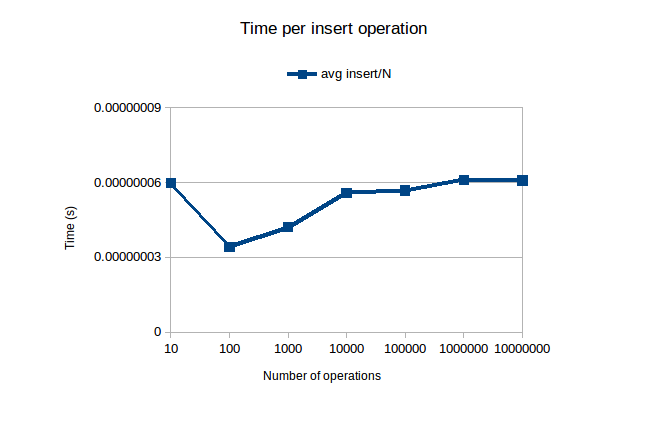
\includegraphics[width=15cm]{Time_per_insert_fibonacci.png}  
  \caption{Time per insert operation in Fibonacci Heap}
  \label{fibonacci-insert-graph}
\end{figure}

\begin{figure}[h]   
  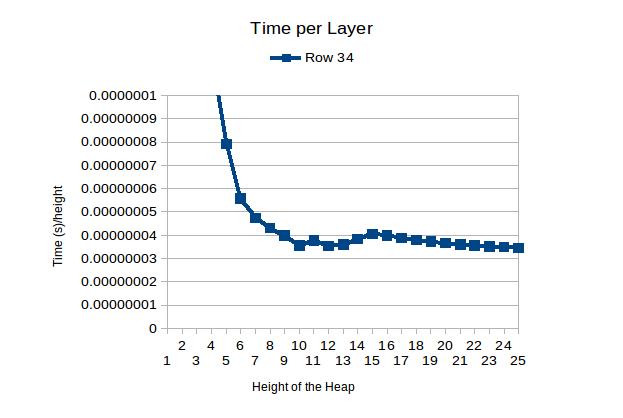
\includegraphics[width=15cm]{Time_per_layer_binary.png}
  \caption{Time per layer in Binary Heap}
   \label{binary-insert-layer-graph}
\end{figure}

\begin{figure}[h]    
  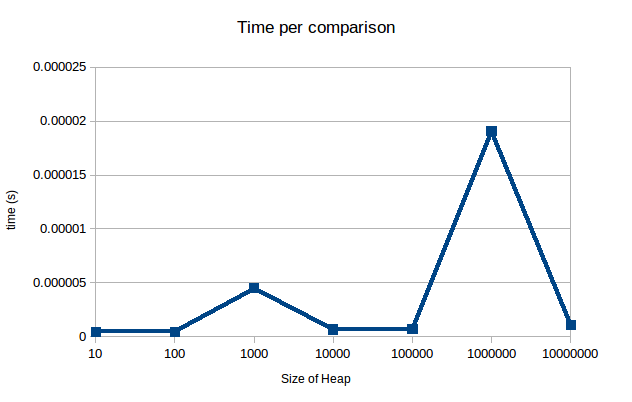
\includegraphics[width=15cm]{Time_per_comparison_binary.png}
  \caption{Time per comparison in Binary Heap}
  \label{timepercompbin}
\end{figure}

\begin{figure}[h]    
  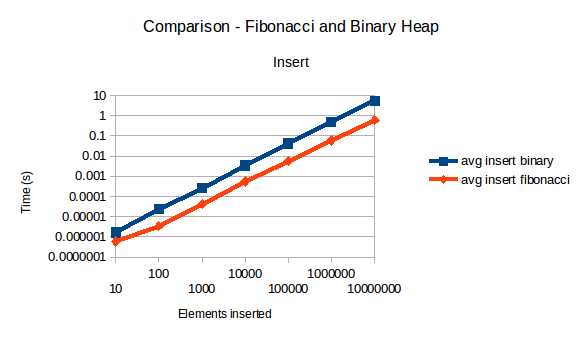
\includegraphics[width=15cm]{Time_insertion_comparison.png}
  \caption{Comparing insertions, Fibonacci against Binary heap}
  \label{timeinscomp}
\end{figure}

\begin{figure}[h]    
  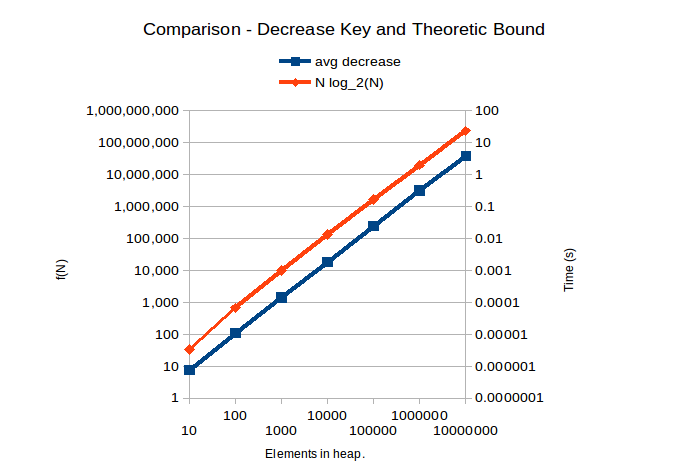
\includegraphics[width=15cm]{Decrease_key_bound_binary.png}
  \caption{Decrease key compared against theretic bounds in Binary heaps}
  \label{binary-decrease-key-graph}
\end{figure}

\begin{figure}[h]   
  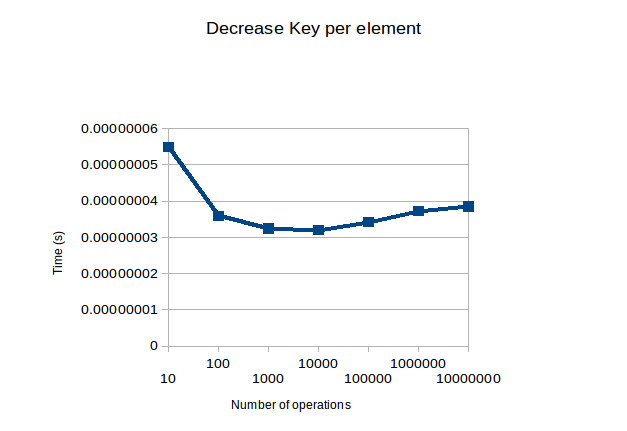
\includegraphics[width=15cm]{Decrease_key_per_element_fibonacci.png}
  \caption{Decrease key per element in Fibonacci Heaps}
  \label{fibonacci-decrease-key-per-element}
\end{figure}

\begin{figure}[h]    
  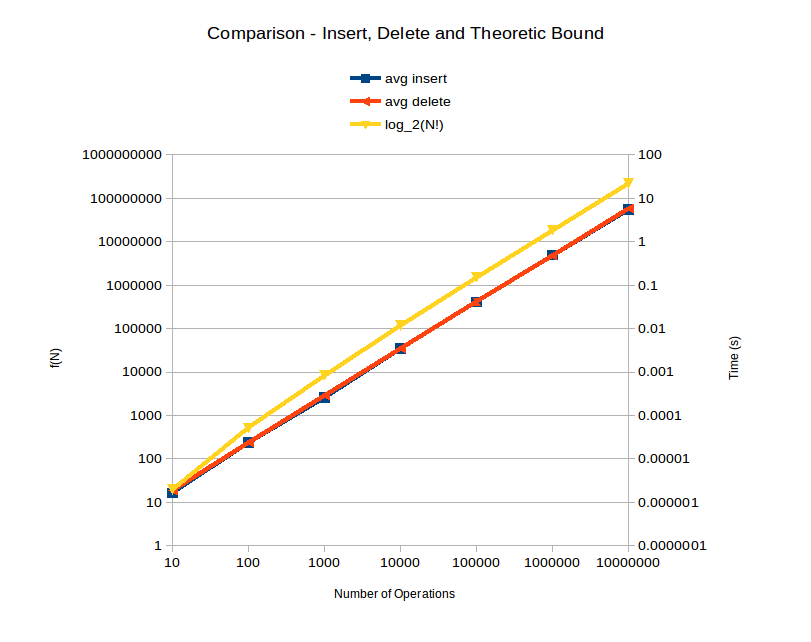
\includegraphics[width=15cm]{Delete_bound_binary.png}
  \caption{Comparing insertions, deletions against theretic boudns in Binary heap}
  \label{delboundbin}
\end{figure}

\begin{figure}[h]    
  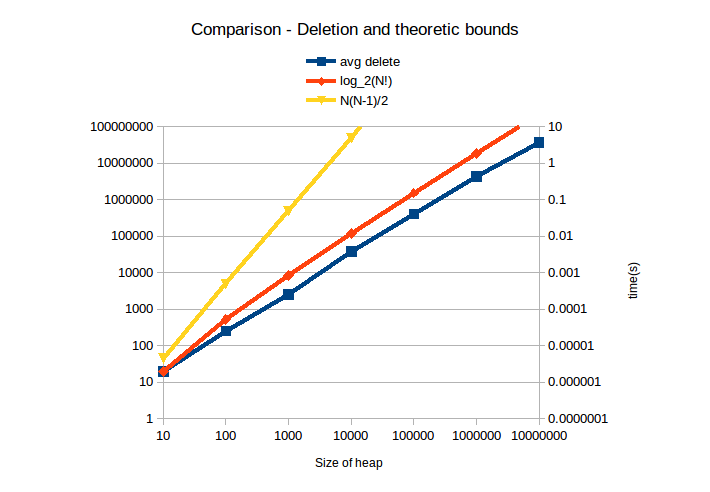
\includegraphics[width=15cm]{Delete_bound_fibonacci.png}
  \caption{Comparing deletions against theoretic bounds in Fibonacci Heaps}
  \label{fibonacci-delete-min-graph}
\end{figure}

\begin{figure}[h]    
  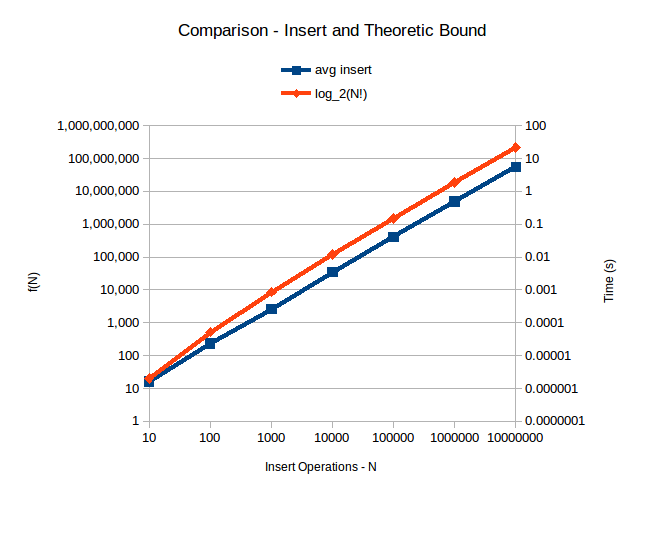
\includegraphics[width=15cm]{Insert_theoretic_bound_binary.png}
  \caption{Comparing insert operations and theoretic bound in Binary Heaps}
  \label{binary-insert-accumulative-graph}
\end{figure}

\begin{figure}[h]    
  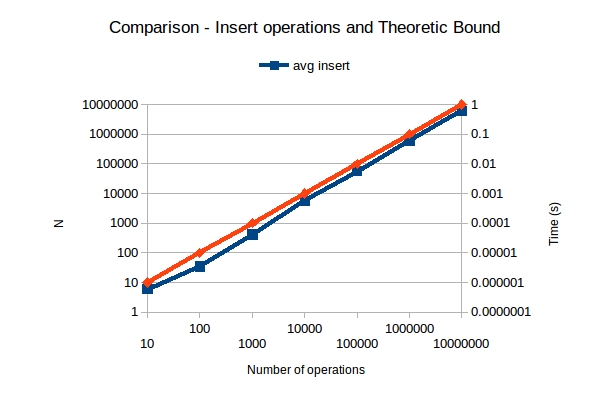
\includegraphics[width=15cm]{Insert_theoretic_bound_fibonacci.png}
  \caption{Comparing insert operations and theoretic bound in Fibonacci Heaps}
  \label{instheoreticboundfib}
\end{figure}

\begin{figure}[h]   
  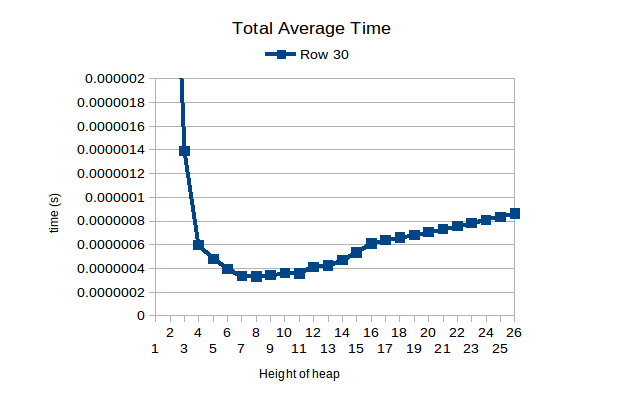
\includegraphics[width=15cm]{Total_time_binary.png}
  \caption{Time of running Binary Heap's insert method on a heap of given height.}
  \label{timeinsbin}
\end{figure}



\end{document}
